\chapter{Discussion}

\Ab{NILM} is an area of research that is gaining a lot of attention due to the more complex smart grid structures. Some of the challenges in the smart grid is that there are not just one \df{generator} of electricity, and a series of \dfs{customer}. There can be multiple of both, and some households contains solar panels, or other energy producing technologies that makes them bout produce and consume energy at different times. This creates challenges for some of the \ab{NILM} applications, as it can camouflage the true power consumption of the houses. The same problem can be created by battery devices, which can mask an appliance power demand. Some of these problems can be observed by monitoring the data quality.

\section{Creating High Quality Measurements}
When monitoring the the data quality as in Chapter~\ref{Sec:DataQuality} a range of problems when collecting consumption data can be detected. When observing the collection of SmartHG data there were two error groups that reviled itself. The one was equipment failure. Both failure for a specific meter, or the server was detected. The second is the houses that exhibit masking behaviour. By looking at the information collected by the sub-meters and comparing it with the main meter data it is possible to detect the masking behaviour created by devices such as solar cells or backup batteries. This will often make it look like the house uses less energy, than recorded by the sub-meters. 

By detecting the errors during the measurement period it is possible to correct some of the errors. This creates better and cleaner measurements. By looking at the measurements \df{activity}, it is possible to find inactive and active areas. This can be used to find active and inactive periods of the devices. These periods can be used to create a more direct training of the statistical models used to do appliance disaggregation. Finding periods in the data where only one single appliance have an ON/OFF cycle, without any other appliance changes state, have shown to be an important training technique. This technique is mostly relevant if sub-meter information is not available. Utilizing the information obtained about the \df{activity} in the quality analysis can help find such spots.

One of the big challenges in a \ab{NILM} application is the amount of devices that are operating on the same power line. A model that needs to disaggregate a signal containing many devices preforms worse than one where there only are few devices. It is therefore beneficial to look at the power usage of each phase individually. By using this separation can the \df{complexity} of the models be reduced greatly, which is shown to increase performance. 

Having these points in mind when measuring data at the \df{customer}, can potentially create a better dataset. A dataset could also improve by supplying information about what devices that are not measured in a research study. If a list of devices in the household was supplied with the measurements it is possible to better gesture about the \df{background consumption} created by the other devices. This kind of information would also be beneficial for methods based on unsupervised learning~\citep{RefWorks:19}. 

\section{Capability Of NILM}
In cases focused around selected appliances have \ab{NILM} shown to be quite effective. But when seeing \ab{NILM} as a tool to disaggregate a whole household appliances, there are still many challenges. Generally it is easy to detect the top consumers in a household. The big consumption increases the chances of a unique power draw pattern. The more unique power draw pattern the easier it is to detect the appliance. The majority of devices in a household only consume a small amount of the total energy. These devices are hard to disaggregate. This is because the power draw pattern for the devices is relatively similar. This causes the device disaggregation models to interfere with each other under the disaggregation process. The result indicates that sometimes some of the events from one device are classified to the wrong devices. 

Much research have been focused on solving this problem. The general concept behind all the solutions are to find other features than the static power draw that can create uniqueness. One approach is to use the difference between the voltage and current usage of the devices, known as the power factor. The power factor can indicate if a load is inductive, capacitive or resistive in nature. One other approach is to sample at high rates in the kHz range. This can supply information about transients, harmonics or noise that can be used to detect uniqueness.

The solutions most commonly used today focus on techniques that uses low sample rates, in the sub 1 Hz range. This is due to the fact that most smart meters are capable of delivering data at these rates. A new type of meter must be developed in order to utilize the benefits that higher sample rates would create. This meter must either sample/transmit the data at higher rates, or process the data on sight and transmit the results. This is a costly process, since a new meter must be developed and installed in the households. By including this type of capabilities in the next generation of smart meters it would be possible to advance the \ab{NILM} research area. This would increase the businesses opportunities for consumer applications that utilizes \ab{NILM} techniques. 

\section{NILM Deployment}
In the current state can \ab{NILM} only deliver a very general picture of the top consumers. What type of devices that is the top consumers is different from country to country. In countries that get hot in the summer, is the air condition at the top of the list. In countries that are cold and have a rocky underground uses a lot of power on electric heading. The difference in consumption culture around the world makes it hard to cross compare results between datasets. This makes it hard to determine which solutions are most suited for a desired country. 

When validating only by looking at the F1 and accuracy scores the results seems promising. When an appliance have a 0.60 F1 score, it generally means that the ON periods was guessed correctly 60\% of the time. This still leaves 40\% of the ON time to be wrongly allocated. The wrong allocations can be both be ON events that are missed and ON events wrongly introduced. This gives the same F1 score, but can make a difference in an application. This is illustrated in Figure~\ref{fig:TVEVENT}, where two versions of the same event signal is shown.  

\begin{figure}[H]
\begin{picture}(0,200)
\put(0,0){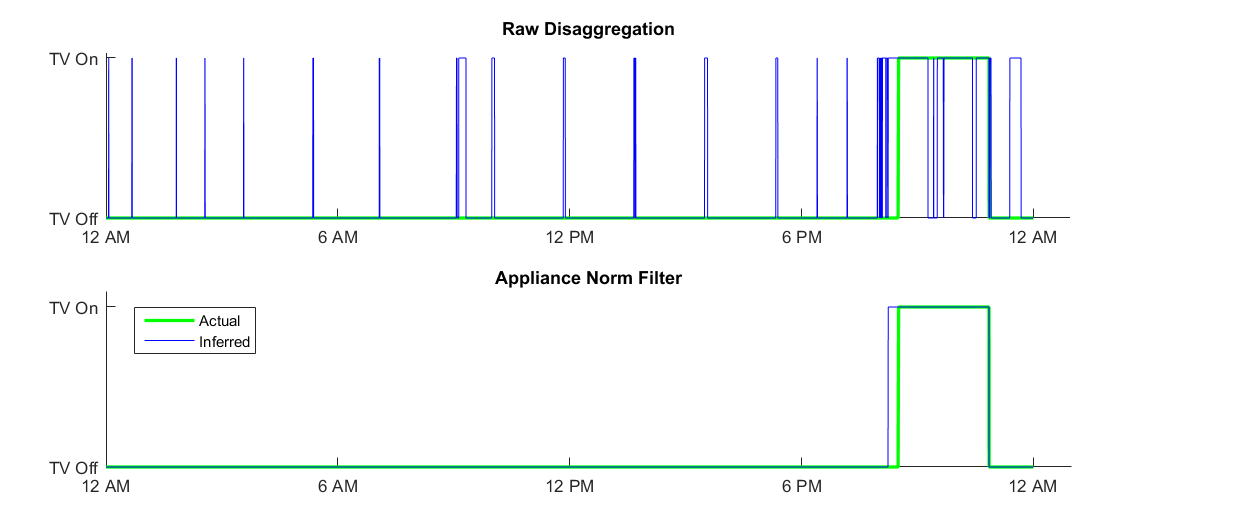
\includegraphics[width=1\textwidth]{billeder/F1vsnormF1.png}}

\put(400,140){F1 $= 0.6656$}
\put(400,130){Accuracy $= 0.5346$}

\put(400,50){F1 $= 0.6866$}
\put(400,40){Accuracy $= 0.5487$}

\end{picture}
\caption{TV event detection.}
\label{fig:TVEVENT}
\end{figure}

The "Raw Disaggregation" is before applying a simple \df{norm filter}. The second illustration is after the \df{norm filter}. The \df{norm filter} used is the same as in in Section~\ref{sec:NormFilter}. Visually the difference between the two signals is huge. The signal after the norm filter is much better than the signal prior to the norm filter. When looking at the F1 and accuracy scores of the two signals, the norm filter have only improved the signal with approximately 2\%.  

This raises the question: \textit{is the F1 score a good indicator, and how high does the score need to be before it is application ready?} The F1 score seems to be generality adopted due to its simplicity and and acceptance in other areas of binary classification~\citep{RefWorks:35}. The F1 score required for an acceptable application can be dependent on many aspects. During the experiments, applications with a F1 score lower than 0.8 was generality influence much by interference from other devices. Where F1 scores higher than 0.8 could be filtered more easily, and gave more intuitive correct results.  

The conclusion being that a functioning \ab{NILM} solution, capable of detecting even little consumers, requires commitment. A successful system will require the metering company to develop, or at least install, a meter capable of high speed data collection or processing. Furthermore must the residents have an interest in helping improving the accuracy, in order to get the best results. This could be done by registering appliances on a smart-phone or tablet as suggested by Weiss~\citep{RefWorks:23}.
\newpage
\section{NILM Privacy Concerns}
Chapter~\ref{sec:CaseStudy} shows that it is possible to gesture about the TV habits of a household. Potentially can the usage pattern for any appliance be derived using \ab{NILM} techniques. Researchers have shown that even the current movie shown on a TV can be deduced by looking at the power profile~\citep{RefWorks:39}. With \ab{NILM} techniques it is more or less possible to track the behaviour of a residential household~\citep{RefWorks:37}.

This kind of possible surveillance raises some privacy concerns. Some simple techniques can be used to mask the appliances from a NILM applications, to improve privacy. It have been shown that down-sampling the consumption signal makes it harder for the \ab{NILM} algorithms. Quantifying the signal by rounding it to a multiple of a pre-defined quantization factor also helps mask signals. Averaging the consumption signal over a time period is also shown to have a masking effect~\citep{RefWorks:40}. Common for all these techniques are that they must be actively build in the meter and transfer mechanisms to mask the appliance data. This will only be the case if the utility companies have the same privacy concerns as the \df{customer}. 

Another approach is to use \ab{NILL}[non-intrusive load leveling] to mask the appliance signals. \Ab{NILL} is a technique where a capacitive device like a battery is used to store energy. This energy is used to camouflage power signatures from the household~\citep{RefWorks:36}. 

\begin{figure}[H]
\centering
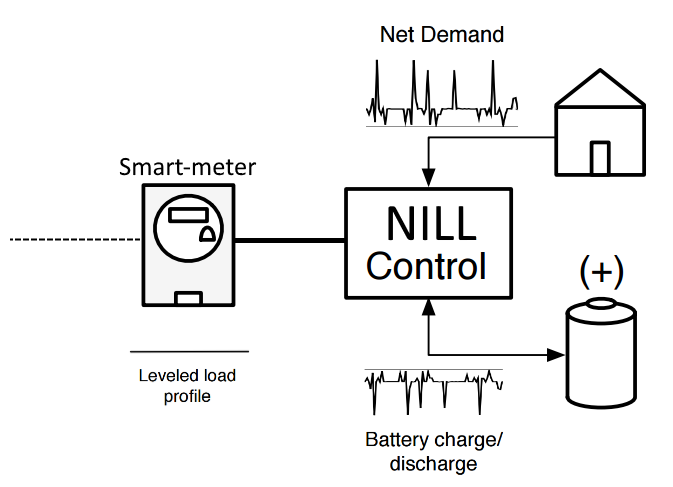
\includegraphics[width=0.5\textwidth]{billeder/NILLILU.png}
\caption[NILL illustration.]{NILL illustration. Inspired by~\citep{RefWorks:36}.}
\label{fig:NILL}
\end{figure}

This principle is illustrated in Figure~\ref{fig:NILL}. A \ab{NILL} solution can be installed after the smart meter and can provide privacy, without the consent of the electricity utility providers.

At the current state of \ab{NILM} is the technology not accurate enough to make reliable detailed surveillance of the household residents. But still advanced enough to raise some privacy concerns. There are many benefits with advancing the possibilities of NILM. Many services can be developed that can support and help the resident. Some of the possibilities are in saving systems and home automation. This systems could greatly benefit the resident of the household. Electronic companies could also benefit from getting accurate user statistics for their devices. But advancing the technology in this direction would also serve to expose the privacy of the home. This raises the questions about who are allowed accesses such sensitive information, and for what purposes?